\documentclass[10pt,a4paper]{article}
\usepackage[utf8]{inputenc} % para poder usar tildes en archivos UTF-8
\usepackage[spanish]{babel} % para que comandos como \today den el resultado en castellano
\usepackage{a4wide} % márgenes un poco más anchos que lo usual
\usepackage[conEntregas]{caratula}

\usepackage{graphicx} % figuras
\usepackage{subfigure} % subfiguras

\begin{document}

\titulo{Trabajo Práctico II}
\subtitulo{Estudio comparativo de performance de implementaciones de una simulación de flujo de fluidos en C y en ASM x86-64 con procesamiento vectorial}

\fecha{\today}

\materia{Organización del Computador II}
\grupo{Grupo: Ariane 5}

\integrante{Greco, Luis}{150/15}{luifergreco@gmail.com}
\integrante{Hertzulis, Nicolás}{811/15}{nicohertzulis@gmail.com}
\integrante{Ramos, Ricardo}{841/11}{riki\_german@yahoo.com.ar}
% Pongan cuantos integrantes quieran

\maketitle

\tableofcontents

\newpage

\section{Introducción}
Introducción: Describe lo realizado en el trabajo práctico. (y si quedó algo sin realizar)


\section{Desarrollo}
El código fuente de la simulación está escrito en lenguaje C y el compilador utilizado es $GCC$. Para las funciones de C \textit{Solver Lin Solve}, \textit{Solver Set Bnd} y \textit{Solver Project} hicimos implementaciones alternativas escritas en el lenguaje ensamblador de la familia de procesadores Intel x86-64. Las instrucciones vectoriales en lenguaje ensamblador utilizan registros de 128 bits. Los estados de la simulación se representan mediante matrices de números decimales de punto flotante de precisión simple (32 bits). Los algoritmos asumen que todas las matrices en una ejecución particular constan de $n\ +\ 2$ filas y $n\ +\ 2$ columnas con $n\ \geq\ 4$ y $n$ múltiplo de 4. A continuación se explica la implementación en ensamblador de las tres funciones.

\subsection{Función Solver Set Bnd}
\par La función $Solver Set Bnd$ se encarga de actualizar los valores del borde. El algoritmo consta de tres partes: el procesamiento de los bordes horizontales (la primera y la última fila de la matriz), el procesamiento de los bordes verticales (la primera y la última columa) y el procesamiento de las esquinas. Los primeros dos se realizan en un ciclo.\newline
\par El procesamiento horizontal consiste en sobreescribir respectivamente las celdas de las filas $0$ y $n\ +\ 1$ con las filas $1$ y $n$ excluyendo la primera y la última celda de las filas. Si el valor del parámetro $b$ es igual a $2$ se cambia el signo del valor a escribir por su contrario, en otro caso se escribe el valor original. La lectura, escritura y cambio de signo se realizan de a $4$ elementos con un registro vectorial, ya que las celdas de cada fila se encuentran contiguas en memoria.\newline
\par El procesamiento vertical consiste en sobreescribir respectivamente las columnas $0$ y $n\ +\ 1$ con las columnas $1$ y $n$ excluyendo la primera y la última celda de las columnas. Si el valor del parámetro $b$ es igual a $1$ se cambia el signo del valor a escribir por su contrario, en otro caso se escribe el valor original. El cambio de signo se realiza de a $4$ elementos con un registro vectorial, pero la lectura y escritura se realizan individualmente porque las celdas no se encuentran contiguas en memoria.\newline
\par El procesamiento de las esquinas consiste en sumar el valor de las dos celdas contiguas a cada esquina (contiguas en la interpretación matricial, no en memoria), luego dividir por dos ese valor y escribirlo en la esquina más cercana a esas celdas. La programación en lenguaje ensamblador implementa un procesamiento alternativo que produce el mismo resultado utilizando instrucciones de asignación ($mov$) y operaciones con enteros en lugar de la operación de punto flotante, que puede generar un error de redondeo. Consideraremos dos casos.\newline
\par El primer caso se da cuando el parámetro $b$ es igual a $1$ o $2$. Si $b$ es $1$ el signo de los valores de los bordes verticales es el opuesto al valor de las celdas de las columnas de origen pero los valores de los bordes horizontales mantienen el signo original. Si $b$ es $2$ se invierte el signo los bordes horizontales y se mantiene el signo de los bordes verticales. Por lo tanto, el proceso consiste en escribir cero en las cuatro esquinas, ya que los dos valores adyacentes a cada una son iguales en módulo y con signos opuestos.\newline
\par El segundo caso se da cuando $b$ tiene otro valor. El proceso consiste en sobreescribir cada esquina con el valor de cualquiera de las dos celdas adyacentes, ya que al no haber cambios de signo estas celdas tienen el mismo valor.\newline
\par El cuerpo del ciclo se implementa con un llamado a función (instrucción $call$) porque si no es demasiado largo para la instrucción $loop$ y se generan errores de compilación.\newline

\subsection{Función Solver Lin Solve}
\par El ciclo principal de la función está formado por dos ciclos: un ciclo que recorre las columnas de las matrices y otro ciclo que recorre las filas. A causa de que las matrices contienen dimensiones múltiplos de cuatro, sin contar con las filas y columnas borde que no se usan en esta función, y los elementos de las matrices ocupan 4 bytes hemos decidido fetchear, fetchear es cargar de memoria, de a cuatro elementos consecutivos de una fila para aprovechar el espacio de los registros $xmm$, que es de 16 bytes, y por lo tanto podemos cargar cuatro elementos en un solo fetch. Así el índice de
las columnas, $i$, queda en un rango entre 1 y $N/4$, donde cada incremento de $i$ representa avance de a cuatro columnas. El ciclo sobre columnas es el primero. Adentro tenemos otro ciclo donde se recorren las filas de a una. \newline

\par Empezamos cargando desde matriz $x$. En cada iteración sobre fila se chequea si la fila es la primera, tal que si es así entonces 
 se realiza $1er$ fetch de cuatro elementos consecutivos desde matriz $x$ en un $xmm$ llamado $xmm\_piso$. Si no es la primera entonces se copian de un registro $xmm$, llamado $xmm\_backup$, que contiene los cuatro resultados de ciclo anterior. Luego realizamos $2do$ fetch de a cuatro de una fila siguiente, en un $xmm$ llamado $xmm\_left$ y avanzamos dos posiciones para un $3er$ fetch de a cuatro en un $xmm$ llamado $xmm\_right$. En la siguiente fila fetcheamos de a cuatro en un $xmm$ llamado $xmm\_techo$. Los elementos cargados desde $x$ forman un bloque de elementos (ver figura 1 $(a)$) de donde vamos a obtener cuatro resultados a partir de seis accesos a memoria. Por otra parte de matriz $x0$ fetcheamos cuatro elementos consecutivos en un $xmm$ llamado $xmm\_x0$.\newline

\begin{figure}[h]
\centering
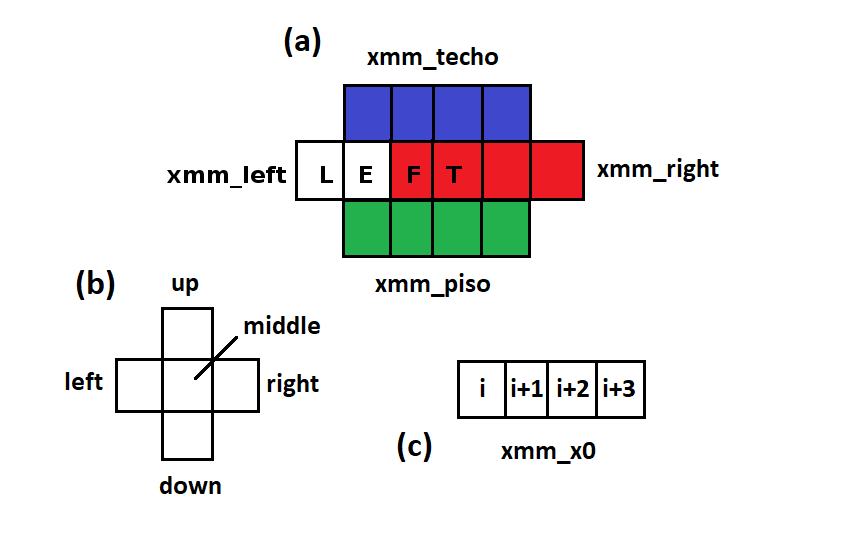
\includegraphics[scale=0.6] {celdas_xmm}
\caption{(a) Bloque de elementos de matriz $x$. (b) Sumandos de $x$ en código $c$. (c) Empacado de elementos de $x0$.}
\end{figure} 

\par Representamos en figura 1 $(b)$ los sumandos de matriz $x$ que aparecen en cuerpo de ciclo principal en código $c$ (ver código $solver\_lin\_solve$ en $solver.c$): up representa al sumando $x[IX(i,j+1)]$, down a $x[IX(i,j-1)]$, left a $x[IX(i-1,j)$ y right a $x[IX(i+1,j)]$. Por último middle representa a sumando $x0[IX(i,j)]$. En bloque de figura 1 $(a)$ vemos que $xmm\_techo$ empaca a los cuatro sumandos up, $xmm\_piso$ empaca a los cuatro down y $xmm\_right$ empaca a los cuatro right de los cuatro puntos centrales del bloque. También vemos, en figura 1 $(c)$, que $xmm\_x0$ empaca a los cuatro middle asociados a los puntos centrales del bloque. La idea que usamos para paralelizar cálculos es sumar los valores de los registros $xmm\_piso$, $xmm\_techo$ y $xmm\_right$ en paralelo obteniendo cuatro sumas parciales. Luego completar la suma alrededor de un punto individualmente, a causa de dependencia de vecino izquierdo, sumando up, down, left y right, comenzando con entorno de primero de los cuatro puntos centrales. Terminar las operaciones sobre ese punto, usando primer middle empaquetado en $xmm\_x0$, y pasar a operar sobre vecino derecho usando como sumando left de este al resultado obtenido. De esta forma se respeta el código $c$ en donde sobre una fila de $x$ los puntos se actualizan hacia derecha, es decir que dependen de sus vecinos izquierdos.\newline
\par Decidimos hacer la conversión de single a double para operar con double float, usando la mayor cantidad posible de bytes, tal que incrementamos la precisión de los resultados.\newline
\par Volviendo al cuerpo del ciclo, una vez que tenemos los datos desempaquetamos con instrucción $cvtps2pd$, que convierte los single en parte baja de $xmm$ fuente a double en $xmm$ destino. Luego shifteamos a derecha con $psrldq$ para acceder a los single de parte alta de los $xmm$ y convertirlos a double.  En este paso obtenemos $xmm\_piso\_low$ y $xmm\_piso\_high$ que corresponden a desempacar a double los 2 single en parte baja y los 2 single en parte alta de $xmm\_piso$ respectivamente. Repetimos este procedimiento con $xmm\_right$ obteniendo $xmm\_right\_low$ y $xmm\_right\_high$. De misma manera desempaquetamos $xmm\_techo$ en $xmm\_techo\_low$ y $xmm\_techo\_high$. Por otra parte se convierten los singles $a$ y $c$ a double en $xmm\_a$ y $xmm\_b$ con instrucción $cvtss2sd$, que convierte escalar single de parte menos significativa de $xmm$ fuente a escalar double en parte baja de $xmm$ destino. Por último convertimos los single de $xmm\_x0$ usando instrucción $cvtps2pd$ en double obteniendo dos $xmm$: $xmm\_x0\_low$ y $xmm\_x0\_high$. También convertimos primer single en $xmm\_left$ a double con instrucción $cvtss2sd$ que convierte single de parte menos significativa de $xmm$ fuente a double en parte baja de $xmm$ destino. Se guarda esto en $xmm\_res$, que usaremos como contenedor de resultados finales.\newline

\par Siguiente paso se suman los dos double de $xmm\_techo\_low$ y $xmm\_right\_low$ guardándose en un $ xmm$ temporal. Luego a estos dos doubles resultado de suma entre techo y lado derecho les sumamos los dos doubles en $xmm\_piso\_low$ obteniendo sumas parciales $x[IX(i+1,j)]+x[IX(i,j-1)]+x[IX(i,j+1)]$ de entorno de dos puntos de $x$. Guardamos esto en $xmm$ llamado $xmm\_sum\_parcial\_low$ y repetimos procedimiento con los $xmm$ de partes altas: $xmm\_techo\_high$, $xmm\_piso\_high$ y $xmm\_right\_high$. Guardamos estos resultados en $xmm\_sum\_parcial\_high$ asociados a otros dos puntos de $x$.\newline

\par Paso siguiente entramos en ciclo que se repite cuatro veces operando sobre doubles de parte baja y obteniendo en cada iteración un resultado a guardar en matriz $x$. Primero se suman escalar de $xmm\_res$ con double en parte baja de alguno de los $xmm\_sum\_parcial$ con instrucción $addsd$ que suma escalares doubles, obteniéndose $x[IX(i-1,j)]+x[IX(i+1,j)]+x[IX(i,j-1)]+x[IX(i,j+1)]$, y guardándose en $xmm\_res$. Entonces se multiplica con escalar $xmm\_a$ usando instrucción $mulsd$, que multiplica escalares double, obteniéndose $a*(x[IX(i-1,j)]+x[IX(i+1,j)]+x[IX(i,j-1)]+x[IX(i,j+1)]) $ y lo guardamos en $xmm\_res$. Luego le sumamos double en parte baja de $xmm\_x0$ obteniendo $x0[IX(i,j)] + a*(x[IX(i-1,j)]+x[IX(i+1,j)]+x[IX(i,j-1)]+x[IX(i,j+1)])$ y lo guardamos en $xmm\_res$. Paso seguido dividimos $xmm\_res$ por escalar $xmm\_c$ con instrucción $divsd$, que divide escalares double, obteniendo $(x0[IX(i,j)] + a*(x[IX(i-1,j)]+x[IX(i+1,j)]+x[IX(i,j-1)]+x[IX(i,j+1)]))/c$ y lo guardamos en $xmm\_res$. En primer iteración $xmm\_res$ contiene sumando left de $1er$ punto central de bloque en figura 1 y al sumar con escalar en parte baja de $xmm\_sum\_parcial\_low$ obtenemos suma de up, low, right y left para ese punto. Realizamos las operaciones restantes y guardamos este resultado en $xmm\_res$ para ser usado como sumando left en siguiente iteración. Finalmente convertimos el resultado en $xmm\_res$ de double a single con instrucción $cvtsd2ss$ y lo movemos a $xmm\_backup$ con instrucción $movss$, que mueve un escalar single a parte baja de $xmm$ destino. Una vez guardado resultado en $xmm\_backup$ shifteamos este registro a izquierda con instrucción $pslldq$, que mueve a izquierda una double quadword, moviendo de a 4 bytes el valor recientemente cargado. De esta manera dejamos espacio para un single en parte baja de $xmm\_backup$ que recibirá a próximo resultado desde $xmm\_res$. En cada iteración de este ciclo shifteamos los registros $xmm\_sum\_parcial\_low$ y $xmm\_x0\_low$ a derecha, con $psrldq$, para acceder a las partes altas de estos y, en caso de haber usado los dos doubles de cada registro pasamos a operar con $xmm\_sum\_parcial\_high$ y $xmm\_x0\_high$.\newline

\par Luego de salir de este ciclo de cuatro iteraciones tenemos en $xmm\_backup$ los cuatro resultados a subir en matriz $x$ pero con las posiciones invertidas por como se cargaron en las iteraciones. Entonces intercambiamos sus posiciones con instrucción $pshufd$ que reubica doublewords en destino con ayuda de un registro temporal. Una vez hecho esto guardamos estos cuatro resultados en matriz $x$, con instrucción $movups$, y saltamos a siguiente fila terminando una iteración de ciclo sobre filas. En próxima iteración no tenemos que cargar de memoria los cuatro resultados obtenidos, ya que los tenemos guardados en $xmm\_backup$, que sobreescribieron fila de $x$ y son requeridos. Al iterar sobre $N$ filas terminamos una iteración de ciclo principal y avanzamos a las siguientes cuatro columnas de $x$ y $x0$. Una vez iterado $N/4$ veces ciclo principal salimos de este con bloque de 
$N\times N$ de $x$ actualizado.\newline

\subsection{Función Solver Project}
\par El algoritmo con el que implementamos esta función se lleva adelande en varias etapas, por un lado los calculos que se hacen dentro del mismo algoritmo, y por otro, los que estan externalizados y llevados a cabo por las otras funciones que fueron implementadas en assembler en este trabajo.\newline

\par Esta implementación sigue la linea del código de la misma función escrito en C, con dos ciclos y llamadas a otras funciones. Como dentro de la función llamamos a $Solver Lin Solve$ y $Solver Set Bnd$ y estos terminan alterando los parametros que utilizamos, necesitamos hacer esos procesamientos en distintos momentos dentro de la ejecución y de ahí la necesidad de hacerlo en dos ciclos.\newline

\par Los calculos que hacemos dentro de la función, trabajan sobre la matriz $div$, con las matrices $u$ y $v$ de solver. Para cada celda de la matriz $div$, vamos a operar con las celdas aledañas (por arriba y por abajo, no las que están en diagonal) a la de la misma posicion de las matrices $u$ y $v$ (tengamos en cuenta que todas estas son matrices de igual dimensión). Notemos que solo podemos realizar estas operaciónes en las celdas de la matriz que no se encuentran en los bordes de la misma. Entonces, vamos a querer hacer estas operaciones con instruciones SIMD. El mayor problema acá se presentó cuando quisimos hacer las operaciones que tomaban las celdas de distintas filas de la matriz. Esto lo resolvimos teniendo 4 punteros, uno a cada celda \textit{aledaña} con la que ibamos a operar, empezando por el primer elemento de nuestra submatriz. Es decir, para el (1,1) tenemos un puntero al (0,1), otro al (2,1), otro al (1,0) y otro al (1,2). Con esto podemos usar SIMD tomando de a 4 elementos, tanto en la matriz que vamos a modificar com en las otras con las que vamos a operar, donde ahora tenemos punteros a los elementos que nos interesan.\newline

\par Cuando tomamos la matriz $div$ (la "principal", o sobre la cual estamos operando), con una instrucción SIMD avanzamos de a 4 celdas. Como la submatriz en la que nos movemos tiene el tamaño de sus filas multiplo de 4 (dato del enunciado), no tenemos que preocuparnos por tomar algún elemento no deseado cuando la función termine de recorrer una fila. Con lo que sí tenemos que tener cuidado es con cómo pasar de una fila a otra, por que en la estructura, entre una fila y otra de la submatriz en la que trabajamos tenemos 2 elementos. Para resolver esto, chequeamos con el tamaño de cada fila (dato) si la terminamos de recorrer. En caso de no haber terminado, seguimos operando sobre la misma fila, y en caso de haber terminado de recorrerla, lo que hacemos es sumar dos posiciónes extras para la próxima iteración, salteandonos así los bordes de la matriz, que no queremos modificar ahora.\newline

\par Ahora lo único que nos restaba hacer en cada ciclo era dejar en cero todas las celdas de la misma submatriz pero de $p$ (o sea, la matriz $p$ sin sus bordes). En nuestra implementación lo hicimos al principio del ciclo (aun que podríamos haberlo hecho en otro momento dentro del ciclo, al no  utilizar la matriz $p$ para nada más a lo largo de ese primer ciclo). Esta matriz la recorremos en conjunto con las demás, al ser exactamente del mismo tamaño de las demás.\newline

\par Con esto termina el primer ciclo de esta función. Ahora llamamos dos veces a $Solver Set Bnd$ para completar los bordes de la matriz, que no los había tocado anteriormente. La llamamos una vez con la matriz $div$ y otra con la matriz $p$. Luego, llamamos a $Solver Lin Solve$.\newline

\par Como podemos observar, estas llamadas a otras funciones modifican los parametros con los que trabajamos. Ahora en el segundo ciclo, trabajamos sobre las matrices $u$ y $v$ de solver (ambas de tamaño (N+$1$) x (N+$1$) ), y al igual que en el ciclo anterior lo que hacemos es recorrer la submatriz de N x N formada por la matriz sin sus bordes. En este caso lo único que cambia respecto del ciclo anterior es que son otras operaciones las que hay que hacer pero no son muy distintas, dado que volvemos a usar esas celdas aledañas. Luego vamos a recorrer las matrices de manera análoga a como hicimos en el primer ciclo.\newline

\par Por último, llamamos a $Solver Set Bnd$ dos veces como hicimos antes, pero en este caso con las matrices $u$ y $v$.\newline


\section{Experimentación}
\subsection{Eficiencia C vs paralelismo simd ASM}
Nuestra hipótesis es que al operar con vectores el código en ASM que usa instrucciones SIMD tendrá menor tiempo de ejecución que código en C. Para averiguar esto evaluaremos los códigos sobre seis tamaños de matrices: 16x16, 32x32, 64x64, 128x128, 256x256 y 512x512. Decidimos usar estos tamaños porque son los que usa la cátedra y nos parecieron que abarcan un buen rango de tamaños. En cada caso repetiremos las ejecuciones cien veces y entonces promediamos los resultados para obtener el desvío estandar. Luego podamos los valores que caigan por arriba de dos veces el desvío estandar calculado, estos valores son llamados outliers. Entonces promediamos los valores no outliers y de acuerdo al porcentaje de valores promediados decidimos si asumir al promedio como representante del comportamiento de los datos o no. \\
Se usa CPU de 2 GB de RAM y 2 GHz de velocidad para correr los experimentos. 
\subsubsection{Función Solver Set Bound}
En cada test establecemos densidad y velocidad inicial. Luego fijamos parámetro matriz en $solver\rightarrow v$ y variamos parámetro $b$. Esto a causa de que el $b$ influye en el resultado de la función: si $b$ es 1 se evalúa una rama en código, si $b$ es 2 se evalúa otra rama y si $b$ no es ni 1 ni 2 se evalúa rama distinta a las anteriores.
El $b$ varía sobre valores 1, 2, 3 y 10.
\subsubsection{Función Solver Lin Solve}
En cada ejecución establecemos densidad y velocidad inicial. Decidimos usar las matrices $solver\rightarrow u$, $solver\rightarrow v$ y variar los otros parámetros porque las matrices sólo aportan sumandos, mientras que los otros parámetros multiplican y dividen.
Evaluaremos con los parámetros $a = 1.0 $, $b$ = 1 y $c = 4.0$, llamado $1erOp$, $a = 0.3$, $b$ = 2 y $c = 2.8$, llamado $2daOp$, $a = 100.0$, $b$ = 3, $c = 20.0$ llamado $3raOp$, $a = -10.0$, $b$ = 10, $c = 0.02$, llamado $4taOp$. Elegimos estos parámetros porque varían en un rango amplio: desde valores decimales, $1erOp$, hasta valores en centenas, $3raOp$.

\subsubsection{Función Solver Project}
Establecemos densidad y velocidad inicial. Hemos medido la función variando parámetros sobre cuatro matrices diferentes: $1erOp$ que comienza con valor (0.1, 0.2) en posición (0, 0) y luego a medida que avanzamos en posiciones se incrementa en uno el valor en posición anterior y se asigna ese resultado a posición actual, $2daOp$ con mismo proceso pero comenzando en (0.2, -100), $3eraOp$ comenzando en (-10, 0.08) y $4taOp$ comenzando en (1000, 2000). Decidimos esos valores por el amplio rango que abarcan.



\section{Resultados}
\subsection{Función solver\_set\_bnd}
\par Se evaluó el código en assembler, llamado ASM, y código C de la función solver set bound sobre seis tamaños distintos de matrices. Al variar parámetro $b$, valores de 1, 2, 3 y 10, se obtienen promedios similares en caso de matriz con tamaño 512x512 (ver tabla), sacando outliers. Los resultados se mantienen alrededor de 18500 ticks para ASM y 54000 ticks para C. 
Repetimos escenario con matriz de tamaño 16x16, variando $b$ en mismos valores que para tamaño 512x512. Aunque se nota 
variación de tiempos entre mediciones (ver cuadro 1) no se nota gran cambio en los resultados, manteniendose el promedio de tiempos C alrededor de 2000 ticks y tiempos ASM alrededor de 350 ticks.\newline
\begin{table}[htbp]
\begin{center}
\begin{tabular}{|l|l|l|}
\hline
  & C & ASM\\
\hline \hline
$solver\_set\_bnd\_100\_16\_b1$ & 2061.989474 & 335.134021\\ \hline
$solver\_set\_bnd\_100\_16\_b2$  & 2081.364583 & 360.896907\\ \hline
$solver\_set\_bnd\_100\_16\_b3$  & 2068.020408 & 376.135417 \\ 
\hline \hline
$solver\_set\_bnd\_100\_512\_b1$  & 56134.061856 & 18529.938144 \\ \hline

$solver\_set\_bnd\_100\_512\_b2$  & 54054.041667 & 19752.25000 \\ \hline

$solver\_set\_bnd\_100\_512\_b3$  &  54835.708333 & 18544.926316 \\ \hline

\end{tabular}
\caption{Tabla de promedios ticks función solver\_set\_bnd para tamaños 16x16 y 512x512.}
%\label{tabla:sencilla}
\end{center}
\end{table}
\par A causa de esto y de que no queremos llenar de gráficas innecesarias hemos decidido fijar el parámetro $b$ en 2 para restantes experimentaciones de función. 
Se muestra en figura 2 promedio de ticks gastado en ejecución de los códigos, donde para cada tamaño los códigos se ejecutaron 100 veces.
\begin{figure}[h]

\centering
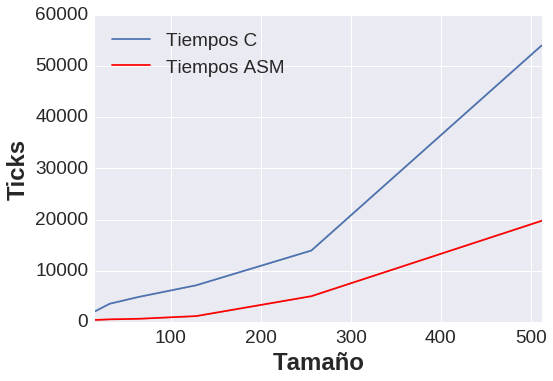
\includegraphics[scale=0.6] {grafica_set_bound}
  
 \caption{Tiempos en ticks de ejecución de código C vs código ASM para función solver\_set\_bnd}
\end{figure} \\
Se ve que el código C gasta más tiempo que código ASM, agrandandose esta diferencia a medida que aumenta el tamaño de matriz.

\subsection{Función solver\_lin\_solve}
\par En este caso hemos variado los parámetros $a,b$ y $c$ para tamaños de matriz 16x16 y 512x512. En la tabla siguiente se muestran los promedios obtenidos sobre datos sin outliers para valores de: $a = 1.0f $y $c = 4.0f$, llamado $1erOp\_a\_y\_c$, $a = 0.3f$ y $c = 2.8f$, llamado $2daOp\_a\_y\_c$, y $a = -10.0f$, $c = 0.02f$, llamado $3raOp\_a\_y\_c$. Los valores de $b$ son: 1, 2, 3 y 10. En el caso de tamaño 16x16 obtenemos que el promedio de tiempos de ejecución sin outliers para código en C está alrededor de los 400000 ticks y para código ASM está alrededor de 300000 ticks. En el caso de tamaño 512x5122 se obtiene que promedio de tiempos C está alrededor de $2.3*e+08$ y tiempos ASM está alrededor de $1.6*e+08 $ ticks.\newline
\begin{table}[htbp]
\begin{center}
\begin{tabular}{|l|l|l|}
\hline
  & C & ASM\\
\hline \hline
$solver\_lin\_solve\_b1\_1erOp\_a\_y\_c\_16$ & 392938.224490 & 236550.530612\\ \hline

$solver\_lin\_solve\_b2\_1erOp\_a\_y\_c\_16$ & 442471.040816 & 252094.406250\\ \hline

$solver\_lin\_solve\_b3\_1erOp\_a\_y\_c\_16$ & 429083.391753 & 253708.344086\\ \hline

$solver\_lin\_solve\_b10\_1erOp\_a\_y\_c\_16$ & 436142.561224  & 261522.363636\\ \hline


$solver\_lin\_solve\_b1\_2daOp\_a\_y\_c\_16$ & 461250.443299 & 369954.084211\\ \hline

$solver\_lin\_solve\_b10\_2daOp\_a\_y\_c\_16$ & 430715.626263 & 352677.979592\\ \hline

$solver\_lin\_solve\_b1\_3raOp\_a\_y\_c\_16$ & 427202.773196  & 262558.585859\\ \hline


$solver\_lin\_solve\_b10\_3raOp\_a\_y\_c\_16$ & 429630.377551    & 237256.265306\\ \hline

\hline \hline 


$solver\_lin\_solve\_b1\_1raOp\_a\_y\_c\_512$ & 2.320231e+08  & 1.576663e+08\\ \hline

$solver\_lin\_solve\_b2\_1raOp\_a\_y\_c\_512$ & 2.364991e+08  &  1.582853e+08\\ \hline

$solver\_lin\_solve\_b10\_1raOp\_a\_y\_c\_512$ & 2.313464e+08   &  1.570360e+08\\ \hline

$solver\_lin\_solve\_b1\_3raOp\_a\_y\_c\_512$ & 2.343117e+08  & 1.585373e+08\\ \hline

$solver\_lin\_solve\_b10\_3raOp\_a\_y\_c\_512$ & 2.337076e+08 & 1.611139e+08\\ \hline

\end{tabular}
\caption{Tabla de promedios ticks función solver\_lin\_solve para tamaños 16x16 y 512x512.}
%\label{tabla:sencilla}
\end{center}
\end{table}
\par Se ve en la cuadro 2 que se repite una proporción de casi el doble de gasto temporal en ejecuciones C respecto a ejecuciones ASM. Entonces decidimos elegir parámetros de $1erOp\_a\_y\_c$, $b = 2$ y las matrices $solver\rightarrow u$, $solver\rightarrow v$.
 Con estos parámetros variamos el tamaño de las matrices y graficamos los tiempos (ver figura 3).
\begin{figure}[h]

\centering
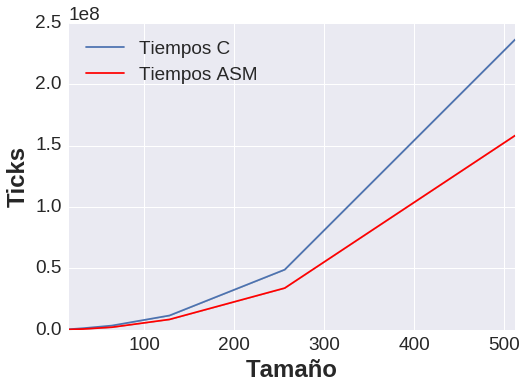
\includegraphics[scale=0.6] {solver_lin_solve}
  
 \caption{Tiempos en ticks de ejecución de código C vs código ASM para función solver\_lin\_solve}
\end{figure}
Se observa notable diferencia de gasto temporal, código C gasta más ticks que ASM.

\subsection{Función solver\_project}
\par Hemos medido la función sobre cuatro matrices diferentes: $1erOp$ que comienza con valor (0.1,0.2) en posición (0,0) y luego a medida que avanzamos en posiciones se incrementa en uno el valor en posición anterior y se asigna ese resultado, $2daOp$ con mismo proceso pero comenzando en (0.09,-100), $3eraOp$ comenzando en (-10,0.08) y $4taOp$ comenzando en (1000,2000). Se evalúan matrices con tamaño 16x16 y 512x512 para observar si hay gran cambio en las proporciones de tiempo al ejecutar código. Se observa en cuadro 3 los resultados y se ve que 
para ambos tamaños el código C gasta alrededor de un tercio más que tiempo gastado por código ASM.\newline
 

\begin{table}[htbp]
\begin{center}
\begin{tabular}{|l|l|l|l|l|}
\hline
  & C &  SD(C) & ASM & SD(ASM)\\
\hline \hline

$solver\_project\_1erOp\_matrices\_16$ & 384948.313131 & 36503.785424 & 271883.232323 & 28601.904704\\ \hline
 
$solver\_project\_2daOp\_matrices\_16$ & 385072.787879 & 34959.635332 & 271078.418367 & 15269.103250\\ \hline

$solver\_project\_3eraOp\_matrices\_16$ & 382180.464646 & 29999.207094  & 273869.231579 & 13431.150139\\ \hline

$solver\_project\_4taOp\_matrices\_16$ & 353107.683673 & 24055.789775    & 259020.680412 & 12374.032677\\ \hline
\hline \hline
 
$solver\_project\_1erOp\_matrices\_512$ & 1.925452e+08 &  1.804747e+06   & 1.584625e+08 & 1.589767e+06\\ \hline

$solver\_project\_2daOp\_matrices\_512$ & 1.939796e+08 &  3.205834e+06   & 1.591681e+08 & 2.147394e+06\\ \hline


$solver\_project\_4taOp\_matrices\_512$ & 1.938470e+08 & 2.764452e+06   & 1.670031e+08 & 8.623912e+06\\ \hline

\end{tabular}
\caption{Tabla de promedios ticks función solver\_project para tamaños 16x16 y 512x512. SD es desvío estandar.}
%\label{tabla:sencilla}
\end{center}
\end{table}

\par A causa de que al variar la matriz obtenemos resultados similares, alrededor de 380000 ticks en código C y alrededor de 270000 en asm para tamaño 16x16 (ver tabla), hemos decidido evaluar los códigos sobre matriz $1erOp$. En la gráfica se muestran los promedios para distintos tamaños (figura 4).\newline

\begin{figure}[h]
\centering
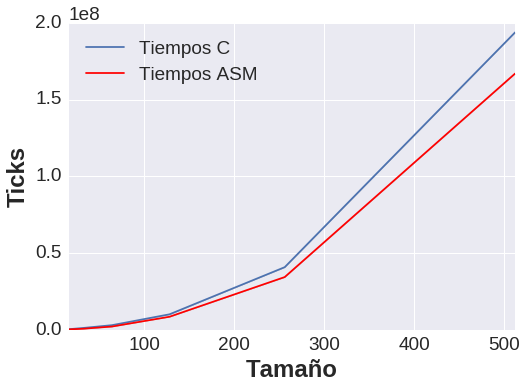
\includegraphics[scale=0.6] {solver_project}
   \caption{Tiempos en ticks de ejecución de código C vs código ASM para función solver\_project}
\end{figure}

\par Observando la gráfica vemos que en este caso la diferencia de tiempos no es tan grande. Notamos que el código de la función hace repetidamente llamadas a las otras funciones: solver\_set\_bnd y solver\_lin\_solve. Se ve que a medida que el tamaño de matriz aumenta las curvas que representan los gastos de tiempo tienden a separarse.






\section{Conclusión}
\par 
Notamos que uno de los principales beneficios de implementar nuestro codigo en Assembler en lugar de hacerlo en C, es la posibilidad de paralelizar operaciones mediante instrucciones SIMD.
En ese sentido, el primer desafío que nos encontramos al hacer este trabajo, fue intentar hacer uso de estas instrucciones siempre que sea conveniente, de manera de agilizar la ejecución de nuestro código lo más posible.\\
Esto lo pudimos llevar a cabo especialmente al trabajar con vectores, ya que al ubicarse en posiciones de memoria contiguas, en cada fetch podíamos leer y procesar más de una posicion de memoria por acceso a la misma. De otra manera, hubiera sido inevitable tener un acceso a memoria por cada operación. Fue en estas operaciones donde pudimos sacarle mayor jugo al uso de este tipo de instrucciones.\\
Por otro lado, también nos encontramos con situaciones donde no nos resultaba conveniente su uso, en las operaciones secuenciales.
En estos casos necesitabamos para cada operación un resultado proveniente de una operación previa, lo que nos impedía implementarlas de forma paralelizada. En este caso no tenía sentido utilizar operaciones SIMD.\\

%\par La primera problemática encontrada fue identificar en qué casos se puede paralelizar el procesamiento y en cuáles no. Notamos que es posible aprovechar instrucciones vectoriales cuando los datos están ubicados en forma contigua en memoria tal que en un fetch levantamos varios datos, evitando múltiples accesos a memoria. También notamos que no siempre se puede obtener resultados en paralelo con vectores. Si el cálculo es secuencial, disminuye el rendimiento del programa, dado que en ese caso no pudimos paralelizar la operación, al necesitar para cada operación el resultado de la anterior.

\par El tiempo de ejecución tiende a mantenerse constante entre las implementaciones de C y ASM empleando instrucciones SIMD, siendo siempre menor la medición de las implementaciones en ensamblador.
Por ejemplo, en un análisis de los gráficos de resultados, se puede observar que, a pesar de la variación del tamaño de las entradas, la proporción de microsegundos se mantiene constante entre C y ASM.\\

\par No es lo mismo una implementación en C que una adaptación a lenguaje ASM. Por ejemplo, al correr demo modo 2 (test), el módulo de la diferencia de cada uno de los resultados obtenidos por implementación ASM y C fue siempre menor que $10^{-4}$ en las pruebas realizadas, sin embargo, esta diferencia nunca fue cero.\\


\par Por otra parte las optimizaciones de compilador, opción $o1$ y $o3$,en nuestro caso no demostraron cambios notables en los resultados respecto a compilar con opción $o0$. Suponemos que esto es a causa de usar tamaños de matrices menores a 600x600.

 
% \par
% Nuestro objetivo era comparar los rendimientos del mismo programa implementado en C  y en Assembler.
%Al convertir floats de precisión simple a doble antes de llevar a cabo operaciones matemáticas.
%Para medir esto, decidimos tomar como medida el módulo de la diferencia de cada uno de los resultados obtenidos en C y Assembler, y en todos los casos obvervamos una diferencia de al menos $10^{-4}$. Esto no nos pareció una diferencia muy considerable, sin embargo no estamos del todo convencidos de la verosimilutud de esta concluisión, al basarse en muestras relativamente reducidas. Con muestras más amplias, podríamos sacar una conclusión más segura.

 

\end{document}
